 \documentclass[0-thesis.tex]{subfiles}

\begin{document}
This chapter presents the background needed to understand the thesis.
Section~\ref{sec:network} introduces the network protocols used and motivates their use
over other protocols in an IoT context. The following section, Section~\ref{sec:suit}
presents and explains the SUIT architecture and information model and their respective
requirements as formulated by the IETF. Finally, Section~\ref{sec:contiki-ng} presents the
Contiki-NG operating system which the updating mechanism will be developed for as well as
the target hardware.

\section{IoT Network Stack}
\label{sec:network}
Network protocols in IoT networks operate under different circumstances compared to
traditional computer networks. Whereas traditional networks enjoy high reliability, high
throughput, and high computational performance IoT networks are defined by their low power
requirements, low reliability, and low computational performance on edge devices. This
posts some constraints on the protocols used in IoT as they must properly handle these
characteristics.

One of the most widely used network protocol stacks today in traditional networks is based
on the \gls{ip}. The stack uses \gls{tcp} as a transportation protocol, usually with
\gls{tls} for security, and a common application layer protocol is \gls{http}. TCP is
however poorly suited for IoT networks as it is a connection based, stateful protocol
which tries to ensure the guaranteed delivery of packets in the correct order. There is
also advanced congestion control mechanisms in TCP which are hard to apply on unreliable
low-bandwidth networks. IoT networks often utilize \gls{udp} as a transport protocol
instead. UDP is also an IP-based protocol but is connectionless and less reliable than
TCP, performing on a best-effort level instead. Despite being less reliable, UDP often
performs better in IoT contexts.

As TLS is based on the same assumptions as TCP it is unsuitable for UDP networks. UDP
networks still need confidentiality and integrity through some means and thus use
\gls{dtls}, which is a version of TLS enhanced for use in datagram oriented protocols.
HTTP can be used over UDP for the application layer, but as HTTP is encoded in human
readable plaintext it is unnecessarily verbose and not optimal for constrained networks.
Instead, \gls{coap} is a common protocol for the application layer in IoT networks. Figure
\ref{fig:stack-comparison} shows the equivalent protocols for IoT network stacks versus
traditional network stacks. 

In this chapter, Section~\ref{ssec:udp} explains UDP and why it is the preferred transport
protocol in IoT networks. Section~\ref{ssec:dtls} briefly explains TLS, why it is
unsuitable for IoT networks, the differences between TLS and DTLS and why DTLS is used
instead. Section~\ref{ssec:coap} describes the CoAP protocol. Lastly,
Sections~\ref{ssec:est-coaps} and \ref{ssec:ace} briefly introduces the EST-coaps protocol
and ACE framework, enabling asymmetric cryptography and authorization in an IoT context.

\begin{figure}
    \begin{bytefield}[bitformatting=\small, bitwidth=1.1em]{30}
        \bitbox[]{12}{IoT stack} & \bitbox[]{4}{} & \bitbox[]{12}{Traditional stack}\\
        \bitbox{12}{CoAP(s)} & \bitbox[]{4}{$\Longleftrightarrow$} \bitbox{12}{HTTP(S)}\\
        \bitbox{6}{UDP} & \bitbox{6}{DTLS} & \bitbox[]{4}{$\Longleftrightarrow$} \bitbox{6}{TCP} & \bitbox{6}{TLS}\\
        \bitbox{12}{IPv6} & \bitbox[]{4}{$\Longleftrightarrow$} \bitbox{12}{IPv4 or IPv6}\\
        \bitbox{6}{IEEE 802.15.4} & \bitbox{6}{6LoWPAN} & \bitbox[]{4}{$\Longleftrightarrow$} \bitbox{12}{IEEE 802.15.4}\\
        \bitbox{12}{IEEE 802.15.4} & \bitbox[]{4}{$\Longleftrightarrow$} \bitbox{12}{IEEE 802.15.4}\\
    \end{bytefield}
    \caption{Comparison of network stacks between IoT networks and traditional networks.}
    \label{fig:stack-comparison}
\end{figure}

\subsection{UDP}
\label{ssec:udp}
UDP is a stateless and asynchronous transfer protocol for IP \parencite{rfc768}. It does
not provide any reliability mechanisms but is instead a best-effort protocol. It also does
not guarantee delivery of messages. For general purposes in unconstrained environments TCP
is usually the favored transport protocol as it is robust and reliable, but in
environments where resources are scarce and networks unreliable, a stateful protocol like
TCP could face issues. Since TCP wants to ensure packet delivery, it will retransmit
packages generating a lot of traffic and processing required for a receiver. Also, if the
connection is too unstable TCP will not work at all since it can no longer guarantee the
packets arrival. The best-effort approach of UDP is favorable in these situations, in
addition to UDP being a lightweight protocol requiring a smaller memory footprint to
implement.

Figure~\ref{fig:udp-header} shows the UDP header format. The source port is optional, the
length denotes the length of the datagram (including the header), and the checksum is
calculated on a pseudo-header constructed from both the IP header, UDP header, and data.
UDP headers are minimalist which shows the point of it being a lightweight protocol with
not many features available.

\begin{figure}
    \begin{bytefield}[bitformatting=\small, bitwidth=1.1em]{32}        
        \bitheader{0-31}\\
        \bitbox{16}{Source port} & \bitbox{16}{Destination port}\\
        \bitbox{16}{Length} & \bitbox{16}{Checksum}\\
        \bitbox[tlb]{32}{Data octets $\dots$}\\
    \end{bytefield}
    \caption{The UDP header format.}
    \label{fig:udp-header}
\end{figure}

\subsection{DTLS}
\label{ssec:dtls}
DTLS is a protocol which adds confidentiality and integrity to datagram protocols like UDP
\parencite{rfc6347}. The protocol is designed to prevent eavesdropping, tampering, or
message forgery. DTLS is based on TLS, a similar protocol for stateful transport protocols
such as TCP, which would not work well on unreliable networks as previously discussed. The
main issues with using TLS over unreliable networks is that TLS decryption is dependant on
previous packets, meaning the decryption of a packet would fail if the previous packet was
not received. In addition, the TLS handshake procedure assumes all handshake messages are
delivered reliably which is rarely the case in IoT networks using UDP.

DTLS solves this by banning stream ciphers, effectively making decryption an independent
operation between packets, as well as adding explicit sequence numbers. Furthermore, DTLS
supports packet retransmission, reordering, as well as fragmenting DTLS handshake messages
into several DTLS records. These mechanisms makes the handshake process feasible over
unreliable networks. 

By splitting messages into different DTLS records, fragmentation at the IP level can be
avoided since a DTLS record is guaranteed to fit an IP datagram. IP fragmentation is
problematic in low-performing networks since if a single fragment of an IP packet is
dropped all fragments of that packet must be retransmitted, and thus fragmenting at the IP
level should be avoided. Since DTLS is designed to correctly handle reordering and
retransmission in lossy networks, splitting messages into several DTLS records is no
problem, and if one record is lost only that record needs to be retransmitted in a single
IP packet.

In order to communicate via TLS and DTLS, a handshake has to be carried out. The handshake
establishes parameters such as protocol version, cryptographic algorithms, and shared
secrets. The TLS handshake involves hello messages for establishing algorithms, exchanging
random values, and checking for earlier sessions. Then cryptographic parameters are shared
in order to agree on a shared premaster secret. The parties authenticate each other via
public key encryption, generate a shared master secret based on the premaster secret, and
finally verifies that their peer has the correct security parameters.

The DTLS handshake adds to this a stateless cookie exchange to complicate DoS attacks,
some modifications to the handshake header to make communication over UDP possible, and
retransmission timers since the communication is unreliable. Otherwise the DTLS handshake
is as the TLS handshake.

\subsection{CoAP}
\label{ssec:coap}
CoAP is an application layer protocol designed to be used by constrained devices over
networks with low throughput and possibly high unreliability for machine-to-machine
communication \parencite{rfc7252}. While designed for constrained networks, a design
feature of CoAP is how it is easily interfaced with HTTP so that communication over
traditional networks can be proxied. CoAP uses a request/response model similar to HTTP
with method codes and request methods that are easily mapped to those of HTTP. Furthermore
CoAP is a RESTful protocol utilizing concepts such as endpoints, resources, and \gls{uri}.
These features makes it easier to design IoT applications that seamlessly interact with
traditional web services. Additionally CoAP offers features such as multicast support,
asynchronous messages, low header overhead, and UDP and DTLS bindings which are all
suitable for constrained environments.

As CoAP is usually implemented on top of UDP, communication is stateless and asynchronous.
For this reason CoAP defines four message types: Confirmable, Non-confirmable,
Acknowledgment, and Reset. Confirmable messages must be answered with a corresponding
Acknowledgment, this provides one form of reliability over an otherwise unreliable
channel. Non-confirmable messages do not require an Acknowledgment and thus act
asynchronously. Reset messages are used when a recipient is unable to process a
Non-confirmable message.

Since CoAP is based on unreliable means of transport, there are some lightweight
reliability and congestion control mechanisms in CoAP. Message IDs allows for detection of
duplicate messages and tokens allow asynchronous requests and responses be paired
correctly. There is also a retransmission mechanism with an exponential back-off timer for
Confirmable messages so that lost Acknowledgments does not cause a flood of
retransmissions. Additionally, CoAP features piggybacked responses, meaning a response can
be sent in the Acknowledgment of a Confirmable or Non-Confirmable request if the response
fits and is available right away. This also reduces the amount of messages sent by the
protocol.

The length of the payload is dependant on the carrying protocol and is calculated
depending on the size of the CoAP header, token, and options as well as maximum DTLS
record size. Section 4.6 of the CoAP standard says "If the Path MTU [Maximum Transmission
Unit] is not known for a destination, an IP MTU of 1280 bytes SHOULD be assumed; if
nothing is known about the size of the headers, good upper bounds are 1152 bytes for the
message size and 1024 bytes for the payload size" \parencite{rfc7252}.

Since firmware images can be relatively large their size needs to be handled during
transportation, which can be done via block-wise transfers \parencite{rfc7959}. A Block
option allows stateless transfer of a large file separated in different blocks. Each block
can be individually retransmitted and by using monotonically increasing block numbers, the
blocks can be reassembled. The size of blocks can also be negotiated between server and
client meaning they can always find a suitable block size, making the mechanism quite
flexible. Another option of interest is the observe option, which allows a client to be
notified by the server when a particular resource changes. This option can be used in a
pull or hybrid update architecture, meaning the device does not have to continuously poll
the server for a new update.

\subsection{EST-coaps}
\label{ssec:est-coaps}
EST-coaps is a protocol for certificate enrollment in constrained environments using CoAP.
\parencite{est-coaps}. By allowing IoT devices to enroll for certificates, asymmetric
encryption can be used even in a constrained environment. EST-coaps is heavily based on
\gls{est} which was developed for traditional, less constrained networks and is thus
incompatible with the SUIT standard, which is specified to work on very small devices
\parencite{rfc7030}. EST-coaps retains much of the functionality and structure of EST but
modifies it slightly to work over CoAP, DTLS, and UDP instead of HTTP, TLS, and TCP, for
instance by making use of CoAPs block requests and responses to remedy the relatively
large sizes of certificates.

\subsection{ACE}
\label{ssec:ace}
% TODO: Put ACE image here to explain? Better than text?
\gls{ace} is a framework for authorization and authentication for IoT contexts, based on
the OAuth 2.0 framework \parencite{ace}. ACE allows for clients in a network to access
protected resources through authorization tokens. An authorization server is used to
distribute tokens to clients, which they then pass on to resource servers. If a token is
valid and the resource requested matches the level of authority associated with the token,
access to the resource is granted. The framework is flexible regarding topologies, and
clients can independently verify the validity of tokens or ask the authorization server
for more information through an introspection request.

The ACE framework can be used to authorize clients in an IoT context. Authorization is
important and distinct from identification, which can be achieve through for instance a
PKI. As the architecture proposed in this thesis aims to be standardized it should prepare
for different parties assuming different roles in the context of updating devices. Using
authorization tokens is a scalable and configurable way of achieving that.

\section{SUIT}
\label{sec:suit}
The IETF Software Updates for Internet of Things (SUIT) working group aims to define a
firmware update solution for IoT devices that is interoperable and non-proprietary
\parencite{suit}. The working group does not however try to define new transport,
discovery, or security mechanisms making their proposal agnostic of any particular
technology. The solution shall be usable on Class 1 devices, defined by ~10 KiB RAM and
~100 KiB code size \parencite{rfc7228}. The solution may be applied to more powerful
devices, such as the one used in this thesis described in Section~\ref{ssec:firefly}.

Section~\ref{ssec:architecture} presents the SUIT architecture and
Section~\ref{ssec:information-model} presents the SUIT information model.

\subsection{Architecture}
\label{ssec:architecture}
There is an Internet Draft by the SUIT group focusing on the architecture of an IoT update
mechanism \parencite{suit-architecture}. This draft describes the goals and requirements
of such an architecture, although makes no mention of any particular technology. The
overarching goals of the update process is to thwart any attempts to flash unauthorized,
possibly malicious firmware images as well as protecting the firmware image's
confidentiality and integrity. These goals reduces the possibility of an attacker either
getting control over a device or reverse engineering a malicious but valid firmware image
as an attempt to mount an attack.

In order to accept an image and update itself, a device must make several decisions about
the validity and suitability of the image. The information needed comes in form of a
manifest. The next section will describe the requirements posted upon this manifest in
more detail. The manifest helps the device make important decisions such as if it trusts
the author of the new image, if the image is intact, if the image is applicable, where the
image should be stored and so on. This in turns means the device also has to trust the
manifest itself, and that both manifest and update image must be distributed in a safe and
trusted architecture. The draft \parencite{suit-architecture} presents ten qualitative
requirements this architecture should have:

% TODO: Descriptive list instead?
\begin{itemize}
    \item Agnostic to how firmware images are distributed:\\
            The mechanism should not assume a particular technology is used to distributed
            manifests and images, but instead be able to be carried over different
            mediums. This means decisions about formats and distribution methods must not
            rely on features of a particular technology.
    \item Friendly to broadcast delivery:\\
            The mechanism should be broadcast friendly, meaning the mechanism can not be
            reliant on security on the transport layer or below. Also, devices receiving
            broadcast updates not meant for them should not incorrectly apply the update.
    \item Use state-of-the-art security mechanisms:\\
            The SUIT standard assumes a \gls{pki} is in place. The PKI will allow for
            signing of the update manifest and firmware image.
    \item Rollback attacks must be prevented:\\
            The manifest will contain metadata such as monotonically increasing sequence
            numbers and best-before timestamps to avoid rollback attacks.
    \item High reliability:\\
            The act of upgrading an image should not cause the device to break. This is an
            implementation requirement. 
    \item Operate with a small bootloader:\\
            The bootloader should be minimal. This is also an implementation requirement. 
    \item Small parser:\\
            It must be easy to parse the fields of the update manifest as large parser can
            get quite complex. Validation of the manifest will happen on the constrained
            devices which further motivates a small parser and thus less complex
            manifests.
    \item Minimal impact on existing firmware formats:\\
            The update mechanism itself must not make assumptions of the current format of
            firmware images, but be able to support different types of firmware image
            formats.
    \item Robust permissions:\\
            Updates must be authorized before they are applied, and different
            configurations might have different requirements for authorization. The
            architecture should enable a flexible and robust permission model.
    \item Operating modes:\\
            The draft presents three broad modes of updates: client-initiated updates,
            server-initiated updates, and hybrid updates, where hybrids are mechanisms
            that require interaction between the device and firmware provider before
            updating. The thesis will look into all three of these broad classes. Some
            classes may be preferred over others based on the technologies chosen in the
            thesis.
\end{itemize}

The distribution of manifest and firmware image is also discussed, with a couple of
options being possible. The two approaches are shown in
Figure~\ref{fig:manifest-image-combined-distribution} and
Figure~\ref{fig:manifest-image-separate-distribution}. The first figure shows the manifest
and image distributed together to a firmware server. The device then receives the manifest
either via pulling or pushing and can subsequently download the image from the same
server. Alternatively, as shown in the second figure, the manifest itself can be directly
sent to the device without a need of a firmware server, while the firmware image is put on
the firmware server. After the device has received the lone manifest through some method,
the firmware can be downloaded from the firmware server. The SUIT architecture does not
enforce a specific method to be used when delivering the manifest and firmware, but states
that an update mechanism must support both types.

\begin{figure}
    \caption{Distributing both manifest and image through a firmware server.}   
    \label{fig:manifest-image-combined-distribution}
    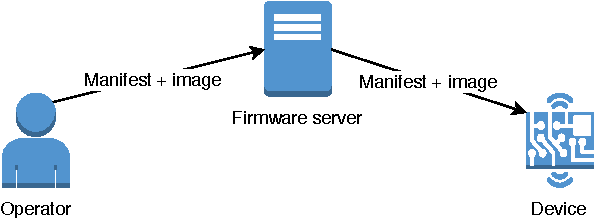
\includegraphics{images/together.pdf}
\end{figure}

\begin{figure}
    \caption{Distributing the manifest directly to the device and image through a firmware server.}
    \label{fig:manifest-image-separate-distribution}
    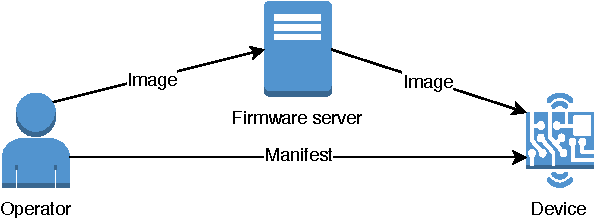
\includegraphics{images/separate.pdf}
\end{figure}

\subsection{Information Model}
\label{ssec:information-model}
The Internet Draft for the SUIT information model presents the information needed in the
manifest to secure a firmware update mechanism \parencite{suit-information-model}. A
manifest is needed for a device to make a decision about whether or not to update itself,
and if the image related to the manifest is valid and its integrity ensured. The draft
also presents threats, classifies them according to the STRIDE model, and presents
security requirements that map to the threats \parencite{stride}. Finally it presents use
cases and maps usability requirements to the use cases in order to motivate the presence
of each manifest element. Note that the information model does not discuss threats outside
of transporting the updates, such as physical attacks.

The proposed mandatory and recommended manifest elements and their brief motivations can
be seen in Table~\ref{tab:manifest-elements}. For the optional elements and more detailed
motivations, use cases, and requirements refer to \parencite{suit-information-model}.

\begin{longtable}[]{@{}lll@{}}
    \caption{The proposed mandatory and recommended manifest elements of the SUIT information model. Adapted from \parencite{suit-information-model}.}
    \label{tab:manifest-elements}\\
    \toprule
    \begin{minipage}[b]{0.23\columnwidth}\raggedright\strut
    Manifest Element\strut
    \end{minipage} & \begin{minipage}[b]{0.26\columnwidth}\raggedright\strut
    Status\strut
    \end{minipage} & \begin{minipage}[b]{0.42\columnwidth}\raggedright\strut
    Motivation/Notes\strut
    \end{minipage}\tabularnewline
    \midrule
    \endhead
    \begin{minipage}[t]{0.23\columnwidth}\raggedright\strut
    Version identifier\strut
    \end{minipage} & \begin{minipage}[t]{0.26\columnwidth}\raggedright\strut
    Mandatory\strut
    \end{minipage} & \begin{minipage}[t]{0.42\columnwidth}\raggedright\strut
    Describes the iteration of the manifest format\strut
    \end{minipage}\tabularnewline
    \begin{minipage}[t]{0.23\columnwidth}\raggedright\strut
    Monotonic Sequence Number\strut
    \end{minipage} & \begin{minipage}[t]{0.26\columnwidth}\raggedright\strut
    Mandatory\strut
    \end{minipage} & \begin{minipage}[t]{0.42\columnwidth}\raggedright\strut
    Prevents rollbacks to older images\strut
    \end{minipage}\tabularnewline
    \begin{minipage}[t]{0.23\columnwidth}\raggedright\strut
    Payload Format\strut
    \end{minipage} & \begin{minipage}[t]{0.26\columnwidth}\raggedright\strut
    Mandatory\strut
    \end{minipage} & \begin{minipage}[t]{0.42\columnwidth}\raggedright\strut
    Describes the format of the payload\strut
    \end{minipage}\tabularnewline
    \begin{minipage}[t]{0.23\columnwidth}\raggedright\strut
    Storage Location\strut
    \end{minipage} & \begin{minipage}[t]{0.26\columnwidth}\raggedright\strut
    Mandatory\strut
    \end{minipage} & \begin{minipage}[t]{0.42\columnwidth}\raggedright\strut
    Tells the device which component is being updated, can be used to
    establish physical location of update\strut
    \end{minipage}\tabularnewline
    \begin{minipage}[t]{0.23\columnwidth}\raggedright\strut
    Payload Digest\strut
    \end{minipage} & \begin{minipage}[t]{0.26\columnwidth}\raggedright\strut
    Mandatory\strut
    \end{minipage} & \begin{minipage}[t]{0.42\columnwidth}\raggedright\strut
    The digest of the payload to ensure authenticity. Must be possible to
    specify more than one payload digest.\strut
    \end{minipage}\tabularnewline
    \begin{minipage}[t]{0.23\columnwidth}\raggedright\strut
    Size\strut
    \end{minipage} & \begin{minipage}[t]{0.26\columnwidth}\raggedright\strut
    Mandatory\strut
    \end{minipage} & \begin{minipage}[t]{0.42\columnwidth}\raggedright\strut
    The size of the payload in bytes\strut
    \end{minipage}\tabularnewline
    \begin{minipage}[t]{0.23\columnwidth}\raggedright\strut
    Signature\strut
    \end{minipage} & \begin{minipage}[t]{0.26\columnwidth}\raggedright\strut
    Mandatory\strut
    \end{minipage} & \begin{minipage}[t]{0.42\columnwidth}\raggedright\strut
    The manifest is to be wrapped in an authentication container (not a
    manifest element itself)\strut
    \end{minipage}\tabularnewline
    \begin{minipage}[t]{0.23\columnwidth}\raggedright\strut
    Dependencies\strut
    \end{minipage} & \begin{minipage}[t]{0.26\columnwidth}\raggedright\strut
    Mandatory\strut
    \end{minipage} & \begin{minipage}[t]{0.42\columnwidth}\raggedright\strut
    A list of digest/URI pairs linking manifests that are needed to form a
    complete update\strut
    \end{minipage}\tabularnewline
    \begin{minipage}[t]{0.23\columnwidth}\raggedright\strut
    Precursor Image Digest Condition\strut
    \end{minipage} & \begin{minipage}[t]{0.26\columnwidth}\raggedright\strut
    Mandatory (for differential updates)\strut
    \end{minipage} & \begin{minipage}[t]{0.42\columnwidth}\raggedright\strut
    If a precursor image is required, this digest condition is needed\strut
    \end{minipage}\tabularnewline
    \begin{minipage}[t]{0.23\columnwidth}\raggedright\strut
    Content Key Distribution Method\strut
    \end{minipage} & \begin{minipage}[t]{0.26\columnwidth}\raggedright\strut
    Mandatory (for encrypted payloads)\strut
    \end{minipage} & \begin{minipage}[t]{0.42\columnwidth}\raggedright\strut
    Tells how keys for encryption/decryption are distributed\strut
    \end{minipage}\tabularnewline
    \begin{minipage}[t]{0.23\columnwidth}\raggedright\strut
    Vendor ID Condition\strut
    \end{minipage} & \begin{minipage}[t]{0.26\columnwidth}\raggedright\strut
    Recommended\strut
    \end{minipage} & \begin{minipage}[t]{0.42\columnwidth}\raggedright\strut
    Helps distinguish products from different vendors\strut
    \end{minipage}\tabularnewline
    \begin{minipage}[t]{0.23\columnwidth}\raggedright\strut
    Class ID Condition\strut
    \end{minipage} & \begin{minipage}[t]{0.26\columnwidth}\raggedright\strut
    Recommended\strut
    \end{minipage} & \begin{minipage}[t]{0.42\columnwidth}\raggedright\strut
    Helps distinguish incompatible devices in a vendors infrastructure\strut
    \end{minipage}\tabularnewline
    \bottomrule
\end{longtable}

As the SUIT architecture tries to be a standardized solution it must account for different
use cases and different combinations of use cases. As a result many of the mandatory and
recommended elements are there to enable certain use cases that might not always be
relevant. This means certain information must be prepared for in advance even if it is not
going to be used in all cases. There is a trade off with flexibility and size, and as the
devices of interest are lightweight it is of interest to reduce the size of the manifest
as much as possible without limiting use cases. With these two considerations in mind, a
manifest for the architecture proposed in this thesis must be designed to facilitate as
many different use cases as possible while keeping sizes to a minimum.

To summarize, the SUIT information model proposes to use a signed manifest that is
distributed to each device in need of an update through some method. The device then
parses the manifest in order to determine if the update is trusted, suitable, and up to
date, with many other optional elements such as if special processing steps or new URIs to
fetch the images are needed. The model does not make assumptions about technology which is
one of the reasons there are optional elements, not all of them are applicable to all
solutions. Nevertheless, the architecture and information model together provides a solid
base on which to design a secure update mechanism for IoT.

\section{Contiki-NG}
\label{sec:contiki-ng}
% TODO: For details on image flipping/bootloaders, talk to Niclas
Contiki-NG is an open-source operating system for resource constrained IoT devices based
on the Contiki operating system \parencite{contiki-ng-github, contiki-github}. Contiki-NG
features an IPv6 network stack designed for unreliable, low-power IoT networks. There are
many protocols implemented in the stack, this thesis will look at UDP and CoAP secured by
DTLS. Beneath IPv6 Contiki-NG supports IEEE 802.15.4 with Time Slotted Channel Hopping
\parencite{ieee-802.15.4}.

The CoAP implementation in Contiki-NG is based on Erbium by Mattias Kovatsch and supports
both unsecured (CoAP) and secured (CoAPs) communication \parencite{low-power-coap}. CoAPs
uses a DTLS implementation called TinyDTLS which handles encryption and decryption of
messages \parencite{tinydtls-github}.

Contiki-NG has a process abstraction which is built on lightweight protothreads
\parencite{protothreads}. Protothreads can be seen as a combination of threads and
event-driven programming. Threads provide a way of running sequential programs
concurrently, enabling the use of flow-control mechanisms. This however requires a
thread-local stack which is too resource heavy on small IoT devices. Event-driven
programming on the other hand does not require a thread-local stack but programs are
limited to computation as callbacks on event triggers, meaning sequential programs are
more difficult to program. Protothreads combine these paradigms in a lightweight way,
keeping the yield semantics of threads and stacklessness of event-driven programming. All
protothreads in a system are run on the same stack, meaning each protothread has a very
low memory overhead, and by providing a conditional blocking wait statement protothreads
can execute cooperatively.

\begin{figure}
    \caption{The state machine of Contiki threads. Adapted from \parencite{contiki-multithreading}.}
    \label{fig:state-machine}
    \begin{tikzpicture}[->,>=stealth',shorten >=1pt,auto,node distance=5cm, semithick]
        \node[initial,state] (A) {Ready};
        \node[state] (C) [below right of=A] {Exited};
        \node[state] (B) [above right of=C] {Running};
    
        \path (A) edge node {stop} (C)
                  edge[bend left=15] node {exec} (B)
              (B) edge[bend left=15] node {yield} (A)
                  edge node {stop} (C);
    \end{tikzpicture}
\end{figure}

Contiki-NGs execution model is event based, meaning processes often yield execution until
they are informed a certain event has taken place, upon which they can act.
Figure~\ref{fig:state-machine} shows the states of the processes and their transitions.
User-space processes are run in a cooperative manner while kernel-space processes can
preempt user-space processes. Examples of events are timers expiring, a process being
polled, or a network packet arriving.

Contiki-NG provides two memory allocators in addition to using static memory. They are
called \texttt{MEMB} and \texttt{HeapMem} and are semi-dynamic and dynamic, respectively.
\texttt{MEMB} is a semi-dynamic allcator that allocates pools of static memory as arrays
of constant sized objects. After a memory pool has been declared, it is initialized after
which objects can be allocated memory from the pool. All objects allocated through the
same pool have the same size. \texttt{HeapMem} solves the issue of dynamically allocating
objects of varying sizes during runtime in Contiki-NG. It can be used on a variety of
hardware platforms, something a standard C \texttt{malloc} implementation could struggle
with. With \texttt{HeapMem} memory can be reallocated and deallocated as if using a normal
\texttt{malloc}.

\subsection{Firefly}
\label{ssec:firefly}
Zolertia Firefly is a supported hardware platform in Contiki-NG and the targeted board for
this thesis. It is a breakout board designed for IoT application development sporting an
ARM Cortex-M3 with 512 KB flash and 32 KB RAM, making it more powerful than the Class 1
devices the SUIT standard specifies as a lower bound. This is not an issue but should be
kept in mind as less capable devices are supposed to be able to use an update mechanism
that is complying with SUIT. Furthermore the board supports IEEE 802.15.4 communication in
the 2.4 GHz band and SHA2 and RSA hardware acceleration \parencite{firefly-datasheet}.

\end{document}